\scanpage{18}
préschémas \deleted{loc. de type fini} \inserted{non ramifiés} séparés sur $S$. \unsure{Seules|Toutes} les \inserted{deux dernières} conditions de modularité se vérifient par des techniques habituelles. \deleted{\unsure{On a des}} Celle au point \uline{générique ne doit pas faire} d'ennuis, avec le calcul habituel d'obstructions.
\margin{\uline{Tout} \uline{\unsure{reste}} à \uline{\unsure{rédiger}}}
\figure{\begin{tikzpicture}[x=1cm,y=1cm]\draw (0,0)--(2.6,.05)..controls(2.85,.06)and(2.85,.26)..(2.85,.45)--(5.2,.5);\draw (.35,-.25)..controls(.43,-.17)and(.47,-.37)..(.57,-.27);\end{tikzpicture}}

Reste le cas où $S$ est local noeth \inserted{irréductible} de dim 1, avec Idéal $J$ annulé par le nilradical, d'où $S_0=V(J)$, et où on dispose de $u_0:X_0\longrightarrow Y_0$ (tel que $u_0\varphi_0=v_0$) et un prolongement $u_\eta:X_\eta-Y_\eta$ ($\eta$ le pt générique de $S$) tel que $u_\eta\varphi_\eta=v_\eta$, $u_{\eta0}=u_{0\eta}$. Question de prolonger $u_0$ en $u$ tel que $u\varphi=v$. \deleted{\unsure{on}} Soient $P(u_0,S),P(u_0,S_\eta);P(v_0,S),P(v_0,S_\eta)$ les prolongements de $u_0$ resp. $v_0$ sur $S$, \deleted{et} de $u_{0\eta}$ resp. $v_{0\eta}$ sur $S_\eta$, d'où le diagramme comm
\figure{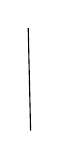
\begin{tikzpicture}[x=1cm,y=1cm]\draw (0,0)--(-.03,1.3);\end{tikzpicture}}
\diagram{\begin{tikzcd}P(u_0,S)\arrow[r]\arrow[d]&P(u_0,S_\eta)\quad *\arrow[d]\\{}_*P(v_0,S)\arrow[r,no head]&P(v_0,S_\eta)\end{tikzcd}} $(1)$
\unsure{d'ens} \unsure{form.} princ. homogènes sous les groupes
\diagram{\begin{tikzcd}\operatorname{Hom}(M_{u_0}^{\unsure{*|\prime}},J)\arrow[r,no head]\arrow[d]&\operatorname{Hom}(M_{u_0},J_\eta)\arrow[d]\\\operatorname{Hom}(M_{v_0},J)\arrow[r]&\operatorname{Hom}(M_{v_0},J_\eta)\end{tikzcd}} $(2)$
Par hypothèse on \unsure{tient} des \unsure{élémts|éléments} aux coins
\mspage{17}
